%%
%% Template chap2.tex
%%

\chapter{Implementing Fingerprint Indexing}
\label{cha:method}

The \HSWAC\ is a significant achievement for the field of automated reasoning.
The theorem prover \beagle\ was designed as a proof of concept; and in its
current form it is certainly capable of demonstrating the
usefulness of the calculus. However, when compared side-by-side with current
state of the art provers like E or Vampire (see Section \ref{sec:proving}) it falls short
of the mark.

The purpose of this project is to make \beagle\ more viable for real-world problems
by implementing recent advancements in automated reasoning; particularly in the
field of term indexing (see Section \ref{sec:indexing}). This chapter covers in
detail how Fingerprint Indexing, a recent technique by \citeN{shulz12} which we described
in Section \ref{sec:fingerprint}, was added to \beagle. This includes analysing
the current structure of the \beagle\ codebase to determine where indexing can
be applied, building the index itself and finally putting the index to active use
in simplifying inference rules. The end of this chapter also details a few
original improvements to Fingerprint Indexing; designed to tailor it to the nuances
of the \HSWAC.

\section{Structure of \Beagle}
\label{sec:initial}

Making any extension to the \beagle\ project (or any sizeable project
for that matter) will obviously require a solid
understanding of the existing codebase. This section provides an overview
of any existing Scala classes which are relevant to the implementation of the Fingerprint Index;
including their structure and any useful existing functionality. 

\subsection{Syntax and Data Structures}

Our term indexer must be able to understand the structure of \beagle's internal
logical objects. Thus the first aspect of \beagle\ we must examine is its existing data structures;
in particular how it expresses first order logic terms.

Figure \ref{fig:expressions} shows how first-order logic terms are stored. Terms
are contained within an Eqn (for Equation) object, which may be ordered ($\to$)
or unordered ($=$). Equations are then directly passed to a Literal container
which stores whether the Equation is positive or negative (true or false). A list
of Literals is maintained for each Clause which are in turn stored in a ClauseSet.
These lists are to be interpreted in \emph{Conjunctive Normal Form} (See Section \ref{sec:fol})
and thus their ordering is not relevant; save for retrieving specific Clauses / Literals.

This structure is fairly typical and quite directly translates the definitions
from Section \ref{sec:fol}. The structure could potentially be shortened by
removing the Equation object and having Literals directly contain the left and right Terms;
but this would be inconsistent with most first-order logic literature and could cause confusion.

\begin{figure}[H]
  \centering
  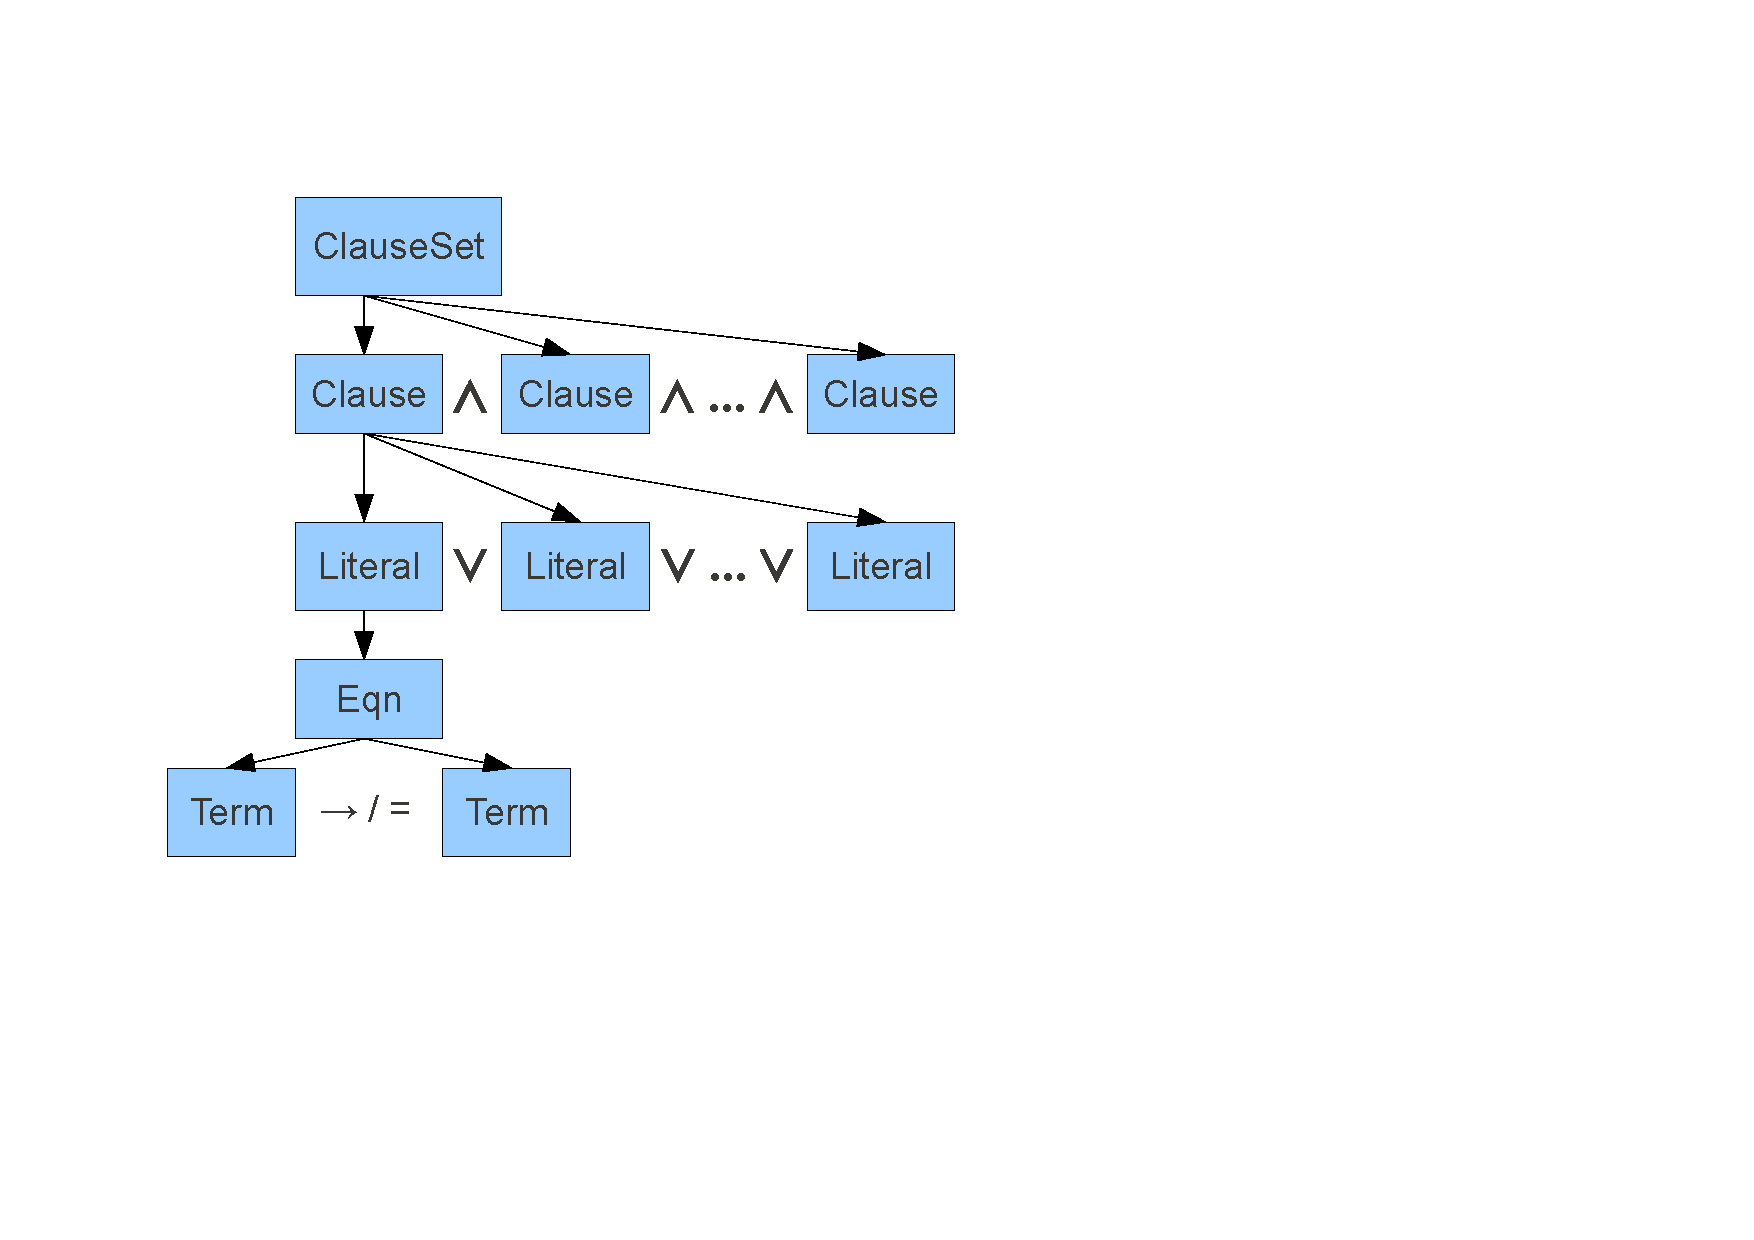
\includegraphics[clip,trim=2.5cm 5cm 13cm 2cm,width=0.75\textwidth]{resources/logicstructure}
  \caption
   {Class structure for internal representation of logical formulae.}
   \label{fig:expressions}
\end{figure}

The object of most concern to our Term Indexer is, naturally, the Term object.
We must be able to pull apart Terms in order to sample them at various positions
to build indexing fingerprints (see Section \ref{sec:fingerprint}). The Term
class itself is actually an \emph{abstract} class with two different primary cases:
\begin{itemize}
\item[] \textbf{FunTerm:} Used to express a function application. Consists of
a function operator and a (possibly empty) list of arguments. Each argument
is another Term object.
\item[] \textbf{Var:} Used to express variables. Variables have a \emph{name}
and a \emph{sort}, used to identify if the variable is in the foreground
or background (i.e. an \emph{abstraction} variable, see Section \ref{sec:hier})
\end{itemize}

For example, the first-order logic term $f(a, g(x))$ (where $x$ is a foreground
variable and other symbols are functions of the appropriate arity) would be expressed as:
\[\text{FunTerm}(f, [\text{FunTerm}(a, []), \text{FunTerm}(g, [\text{Var}(x, FG)])] )\]
Knowledge of this structure will be very useful when we move on to constructing
Term Fingerprints in Section \ref{sec:fpbuild}.

\subsection{Main Inference Procedure}
\label{sec:mloop}

Now that we have a solid understanding of \beagle's relevant data structures
we may move on to examining the main loop of the program. This loop repeatedly
attempts all the inference rules in the {\HSWAC} (see Section \ref{sec:calc})
to generate new information. It also includes some optional rules and optimisations
which are not strictly part of the calculus, but drastically increase performance
in special cases. This includes:
\begin{itemize}
\item \textbf{Simplification:} Removes redundant variables and pre-processes some simple clauses.
Covered in detail in Section \ref{sec:simp}.
\item \textbf{The Split rule:} In some cases the Literals of a Clause may be partitioned
in two; with each partition consistent with our current knowledge. The Split rule allows
us to create a whole new instance of \beagle's main loop, to be run in parallel,
so that we may consider both options. These `branches' may be closed if they return
unsatisfiable.
\item \textbf{The Instantiate rule:} Applies to Clauses with background variables in `\emph{finite domains}'.
If there are finitely many terms which a variable may represent it is sometimes useful
to remove that variable and replace it with one Clause per possible instantiation.
\end{itemize}

In Listing \ref{lst:main} we present a simplified pseudocode version of the main inference loop.
\verb!input ClauseSet! here represents our database of knowledge along with
the \emph{negation} of what we are trying to prove. We input the negation since
we are ultimately looking for a contradiction (i.e. finding that the set is unsatisfiable);
which would then indicate that our original input is always true.
\begin{listing}[H]
\begin{lstlisting}
new := input ClauseSet
old := empty ClauseSet
While new is not empty
   select := Pop a clause from new
   simpl  := |\textbf{Simplify(select,new,old)}|
   If simpl is a tautology:
       Continue
   If simpl is the empty clause:
       return UNSAT
   If one of the Define, Split or Instantiate rules apply to simpl:
       new := new U ApplicableRule(simpl)
       Continue
   old := old U simpl
   Attempt all inference rules:
       new := new U EqualityResolution(simpl)
       new := new U EqualityFactoring(simpl)
       new := new U |\textbf{Superposition(simpl,old)}|
end While
\end{lstlisting}
\caption{Pseudocode for \beagle's main inference procedure.}
\label{lst:main}
\end{listing}

Notice the two bolded subroutines in the main procedure. All other
routines in the main loop require only the input of \verb!simpl!, but these two
also require \verb!old! and/or \verb!new!. This means that their runtime is dependant
on the size of the current ClauseSets; and considering that both sets grow overtime
these two functions are likely to dominate \beagle's runtime.

So \emph{simplification} and \emph{superposition} are the two main areas
we should target for improvement with indexing. This is consistent
with our earlier analysis of the abstract calculus (see Section \ref{sec:shortcomings})
where superposition was identified as the most costly inference rule.

\section{Building the Fingerprint Indexer}
\label{sec:initial}

The first step in adding fingerprint indexing to \beagle\ is creating the indexer
itself; an object which will manage the index and provide functions for adding
to it and retrieving from it.

This Section details the creation of the FingerprintIndex Scala class; containing
all the data types and functions we will need for indexing. This includes building
and comparing term fingerprints, addition and retrieval from a complex index structure
and any auxiliary functions to assist with these computations.

\subsection{Objects and Data Types}
\label{sec:datatypes}

Here we define in detail any data structures which will be a part of our index.
These data structures must be capable of expressing any concepts from
the abstract definition of fingerprint indexing, outlined in Section \ref{sec:fingerprint}
and the original paper \cite{shulz12}.

\subsubsection{Positions}

We implement positions in the simple na\"{\i}ve manner, as a list of
Integers (where Nil, the empty list,  is used to index the top-level term). This
directly reflects our position notation given in Section \ref{sec:terminology}.

\subsubsection{Fingerprint Features}

Fingerprint features are the four possible symbols we get when sampling a term
at an arbitrary position. The meaning of these features is given in Section \ref{sec:fingerprints},
so here we provide only the Scala definition. We essentially only require an
enumerated type for Fingerprint Features, except for the fact that we must be able
to specify a function symbol. Thus we implement this type as four separate case classes
implementing an abstract \verb!FPFeature! class; with one of these classes taking
a function name as a parameter.

\begin{listing}[H]
\begin{scalacode}
/** Pseudo enumerated type for fingerprint features */
sealed abstract class FPFeature
case object FPA extends FPFeature 
case object FPB extends FPFeature
case object FPN extends FPFeature
case class  FPF(val f : String) extends FPFeature
\end{scalacode}
\caption{Data type for the 4 Fingerprint Features \protect\cite[p5]{shulz12}}
\label{lst:featuredata}
\end{listing}

\subsubsection{Term Fingerprints}

With Positions and Fingerprint Features defined it is now very simple
to define the Fingerprint for a Term. We take this as simply a list
of Fingerpint Features, to be acquired by sampling at various Positions. 

\subsubsection{Fingerprint Index}

The final data structure we require is the actual Index itself, a structure
which stores all the indexed terms and their Fingerprints so that they may be later
retrieved.

The na\"{\i}ve method for implementing the Index would be to simply use a HashMap
from Fingerprints to their corresponding Term. This method would however cause
several problems which would make the correct and efficient retrieval of terms impossible.
Fingerprints do not have to be identical in order to match for unification, they will match any
Fingerprints which are compatible with respect to some comparison table (see Section \ref{sec:fingerprints}).
To accommodate this our Index object must store Terms in a way that allows all compatible sets to be
collected together. In Listing \ref{lst:indexdata} we present an algebraic data
type for an Index, structured as a tree of HashMaps. Each Index is either a
collection of Terms (a Leaf) or a mapping from FPFeatures to more Index objects (a Node).

\begin{listing}[H]
\begin{scalacode}
/** Algebraic Data type for our index. Either we are at a leaf
  * (set of terms) or must continue traversal via the map. */ 
sealed abstract class Index
case class Leaf(set: Set[Term])                 extends Index
case class Node(map: HashMap[FPFeature, Index]) extends Index
\end{scalacode}
\caption{Data type for the actual term index. \protect\cite[p7]{shulz12}}
\label{lst:indexdata}
\end{listing}

Note that this Index object does not necessarily take up a significant portion of memory.
All Terms are already stored within the ClauseSet object (See Figure \ref{fig:expressions});
so the Index itself will generally only add a fairly lightweight structure of pointers.


\subsection{Building Term Fingerprints}
\label{sec:fpbuild}
With our required data structures in place we may now begin implementing our
Fingerprint Index proper. There are two main components in this implementation:
adding to the Index and removing from it. A logical first choice is addition; as we
cannot possibly test retrieval until addition is completed. The
first step in implementing addition is creating a function to generate Term Fingerprints; by sampling them
at a fixed set of positions.

A Term's Fingerprint is a list of Fingerprint Features; which we described in Section \ref{sec:fingerprints}
and concretely implemented in Section \ref{sec:datatypes}.
Listing \ref{lst:posextract} provides a function to extract a single Fingerprint Feature from
a Term at a given Position; which is the only non-trivial task in Fingerprint generation.
\begin{listing}[H]
\begin{scalacode}
/** Extract the FPFeature at Position pos of the given Term object. */
def extractFeature(term: Term, pos: Position) : FPFeature = pos match {
  // Reached end of position, check symbol
  case Nil     => term match {
    case t:FunTerm => FPF(t.op) // Found function symbol, return it
    case t:Var     => FPA       // Found variable, return A
  }
  case p :: ps => term match {
    case t:FunTerm => try   {extractFeature(t.args(p), ps)}
                      //Non-existent position, return N
                      catch {case e:IndexOutOfBoundsException => FPN}
    // Found variable BEFORE end of position, return B
    case t:Var     => FPB 
  }
}
\end{scalacode}
\caption{Scala code to extract fingerprint features for matching.}
\label{lst:posextract}
\end{listing}
This code is intended to be a fairly direct implementation of the four
fingerprint features described in Section \ref{sec:fingerprints}
(and \cite{shulz12}). We simply traverse through the Term until
we reach the desired position or we find a variable.

Generating the actual Fingerprint for a Term is now a straightforward process
of repeating this function for each desired Position.

\subsection{Adding Terms to the Index}
Now that we can generate Term Fingerprints we must use them to store Term objects
at the correct position of our Index data structure (see Section \ref{sec:datatypes}).
This is done by following the Index tree mappings for each Fingerprint Feature in
the Fingerprint. Traversing the tree is relatively complex; as at each
level we may need to create nodes in order to continue traversal. Listing \ref{lst:addterm}
presents code for simultaneously traversing the tree while creating Nodes and Leaves.
\begin{listing}[H]
\begin{scalacode}
/** Add a Term into the given Index. Traverses Index tree
  * (adding nodes where needed) and adds Term t to a Leaf set. */
private def add (t:Term, fp:Fingerprint, index: Index):Index =
(fp, index)  match {
  //Reached a leaf at the end of the Fingerprint. Add to set.
  case (Nil,   Leaf(set)) => Leaf(t::set)
  //Still traversing tree. Add new Node or Leaf if necessary
  case (f::fs, Node(map)) => (fs, map.get(f)) match {
    //Mapping exists. Traverse through it.
    case (_,   Some(index)) => {map += (f -> add(t, fs, index))
                                Node(map)}
    //At end of Fingerprint. Create Leaf and add to it
    case (Nil, None) => {map += (f -> Leaf(List(t)))
                         Node(map)}
    //Fingerprint not over. Create Node and continue traversing
    case (_,   None) => {val newIndex:Index = new Node()
                         map += (f -> newIndex)
                         add(t, fs, newIndex)
                         Node(map)}
  }
  case (_, Node(_)) => throw new IllegalArgumentException
                ("Fingerprint is over but we are not at a leaf")
  case (_, Leaf(_)) => throw new IllegalArgumentException
                ("Reached a leaf but Fingerprint is not over")
}
\end{scalacode}
\caption{Code to add a Term to the correct Leaf node of the Index data
structure defined in Section \ref{sec:datatypes}.}
\label{lst:addterm}
\end{listing}
\verb!add! is a recursive function which moves down the Index one step for
each time it is called. Notice that the function takes a Fingerprint as an argument. This argument
should initially be the Fingerprint of the input Term (relative to the Index's list of Positions);
but with each recursive call of \verb!add! we strip off one Fingerprint Feature and follow
its mapping in the Index. Throughout this process we create new Index Nodes as required;
and at the end of the Fingerprint we create (or add to) a Leaf.
In accordance with programming best practices the final two cases in the Listing
throw meaningful error messages in the case of unexpected input.

We may now index an arbitrary Term object; but it is desirable to be able to index
whole Clauses with a single function call. This is done with a straightforward lifting
over the expression syntax tree (Figure \ref{fig:expressions}) : Clauses index all of their Literals, Literals index
their Equation and Equations index each of their two Terms.

\subsection{Retrieving Compatible terms}
\label{sec:retrieve}

Our Index framework is now capable of creating Fingerprints and storing Terms in
its pointer structure. The next task in building our index is allowing retrieval
of any Terms which are compatible with a query Term; relative to some comparison
table.

We will now provide an implementation of the Fingerprint comparison table for unification (Section \ref{sec:fingerprints}).
To compare two Fingerprints with each other we look at them side-by-side and return
\emph{true} or \emph{false} depending on how they match up in the table.
The na\"{\i}ve method for performing this check is to simply check for each possible
entry in the table manually. However, by examining the table more closely we observe
that it can be covered with only four cases:
\begin{enumerate}
\item True if the two Features are equal.
\item True if one of the Features is \textbf{B}.
\item True if one of the Features is \textbf{A}; but the other is not \textbf{N}.
\item False otherwise 
\end{enumerate}
We may implement these four cases in Scala by using the \verb!match! construct
to compare \verb!Set! objects. Using an unordered \verb!Set! object here allows
us to take advantage of the unification table being symmetric by checking both
directions at once. 
\begin{listing}[H]
\begin{scalacode}
 /** Check two Fingerprint features for compatibility based
   * on the unification table (See page 6 of [Shulz 2012]). */
  def compareFeaturesForUnification
         (a:FPFeature, b:FPFeature) : Boolean =
  (a == b) || 
  (Set(a,b) match {
    case x if (x contains FPB) => true
    case x if (x contains FPA) => !(x contains FPN)
    case _ => false})
\end{scalacode}
\caption{Scala implementation of the Fingerprint unification table. \protect\cite[p6]{shulz12}}
\label{lst:unitable}
\end{listing}

To check whether or not two Fingerprints match is now a simple matter of iterating
through the list and checking that each position is a match according to our unification
table check. This side-by-side comparison could potentially be improved by employing
some variety of hashing function; however this sort of improvement does not
apply to our uses for term Fingerprints. Rather than comparing two Fingerprints
side-by-side we are only ever interested in retrieving \emph{all} compatible
terms from our Fingerprint Index (see Section \ref{sec:fpindex}
and Section \ref{sec:datatypes}).

So, rather than individually comparing the Fingerprints of each indexed Term,
we must build a function which traverses the Fingerprint Index tree structure
and collects all compatible terms.

\begin{listing}[H]
\begin{scalacode}
def retrieveCompatible (fp: Fingerprint, index: Index) : TermSet =
(fp, index) match {
//Collect all compatible (Feature,Index) pairs and continue traversal
    case (f::fs, Node(map)) => 
        {for ((k,v) <- map if compare(f, k))
            yield retrieveCompatible(fs, v)}
//Collapse all retrieved sets together with the union operator (:::)
        .foldLeft(Nil:TermSet) ((a,b) => a ::: b)
//Once we reach a Leaf we simply return the compatible set 
    case (Nil, Leaf(set)) => set
    case (_, Node(_)) => throw new IllegalArgumentException
         ("Fingerprint is over but we are not at a leaf")
    case (_, Leaf(_)) => throw new IllegalArgumentException
         ("Reached a leaf but Fingerprint is not over")
}
\end{scalacode}
\caption{Scala code to collect compatible terms from the index.}
\label{lst:retrieve}
\end{listing}

We present \verb!retrieveCompatible! (Listing \ref{lst:retrieve}); which takes
a Term, a Fingerprint and an Index and returns all Terms in the Index which
are compatible with respect to the \verb!compare! function.
\verb!compare! here is a function implementing a Fingerprint Feature comparison
table; such as \verb!compareFeaturesForUnification! from Listing \ref{lst:unitable}.
It can be passed to the Fingerprint Index as part of its configuration
object (see Section \ref{sec:config}).

\verb!retrieveCompatible! works similarly to \verb!add! from Listing \ref{lst:addterm};
recursively stripping off a Fingerprint Feature and traversing the Index tree.
The difference here is that we must `branch off', making a recursive call for
each feature which is compatible (according to \verb!compare!). The \verb!for-yield!
loop takes care of this, returning a list of TermSets which are collected together
by folding the List over the union operation. As in Listing \ref{lst:addterm}, we cover
unexpected input cases with meaningful error messages.


\subsection{Matching with Subterms}

At this stage we have a complete implementation of abstract fingerprint indexing;
as described in Shulz's paper \cite{shulz12}. However, this index is not
quite at the point where it is usable in \beagle\ 
Recall the main superposition rules for \beagle's resolution calculus (Section \ref{sec:calc} and \cite{baum13}).
Notice in particular the condition that $l$ may match against a \emph{subterm}
of $s$ (this condition also exists in the original superposition calculus, Section \ref{sec:supcalc}).
This does not match our current implementation which is only capable of indexing
whole, top-level terms.

Thus our Fingerprint Index must be able to index and collect all possible matches against \emph{subterms}.
To do this we will extend \beagle's Term object with a function to generate all
subterms; along with the position they were extracted from. For variables and constants
this is trivial; we just return the symbol and Nil for the subterm position. For
functional terms however we must collect a list of each argument along with
all subterms of those arguments. Listing \ref{lst:subterms} performs this
operation by recursively finding the subterms of each argument and collecting
them together. 

\begin{listing}[H]
\begin{scalacode}
/** Retrieve all subterms along with their position */
def subtermsWithPos : List[(Term, List[Int])] = 
  (thisterm, Nil) :: (for 
    ((arg,    argpos)    <- args zip args.indices;
     (subarg, subargpos) <- arg.subtermsWithPos)
      yield  (subarg, argpos::subargpos))
\end{scalacode}
\caption{Recursively grab all subterms from a complex term.}
\label{lst:subterms}
\end{listing}
With this extension in place we can index subterms by extending our addition function
(Listing \ref{lst:addterm}) to also add all subterms. This process is straightforward,
we simply create a new function which loops over subterms and adds each one.
This will make the indexer capable of comprehensively indexing all subterms as required.
Our Index however is still unfit for live use in optimising \beagle's inference rules.
This is due to a subtle issue which prevents correct retrieval of all
the information needed by the inference calculus.

\subsection{Current Problems and Term Traces}
\label{sec:problems}
At this stage we have a Fingerprint Index which is capable of comprehensively indexing a Clause
all the way down to individual subterms. However, as previously mentioned,
there is a subtle issue remaining. We shall refer to this issue as \emph{Term Alienation}.
The issue was caught during the process of \emph{Unit Testing} (see Section \ref{sec:unittest}) and relates
to retrieving the Clause structure associated with any Terms retrieved as compatible.

\subsubsection{Term Alienation}
In Listing \ref{lst:indexdata} we presented the actual data structure for storing
indexed Terms. It presented the leaves of this index as simply a set of Term objects.
At this stage we notice that this representation is actually insufficient. \Beagle's
inference rules require knowledge of the Clauses which we are operating on, so
storing only the bottom level Term does not give us enough information to perform any
inferences. This is especially true considering that the stored Term may even
be a subterm of what we actually wish to use for inference.

A first attempt to solve this issue involved giving every object in the expression
tree (Figure \ref{fig:expressions}) a pointer to its `\emph{parent}' expression.
However, ensuring that these pointers were correct at all times proved to be
difficult. Furthermore, the pointers were difficult to use in practice since there
are several steps involved in going from a subterm all the way up to a Clause; and
each object must be collected along the way.

\subsubsection{Term Tracing}

Term Alienation can be better solved by introducing \emph{Term Traces}. A Term Trace
is an object which will be stored alongside any Term in our Index; containing any
required information regarding where the Term originally came from. This includes
pointers to each object higher up in the expression syntax tree (the associated Equation, Literal
and Clause) and the (possibly nil) subterm Position. Term Traces allow us to quickly
and easily retrieve any information required for inferences.
 
It is worth noting at this point that by indexing subterms and adding Term Traces we have
increased the size and complexity of our Index data structure considerably.
This is negligible however since we only introduce pointers rather than whole
copies of expressions. Even in the case of copying data this would be of little
concern since memory is cheap; and we are generally only concerned with speed.

\subsection{Unit Testing with ScalaTest}
\label{sec:unittest}

As with any component of a large software project; it is vital to ensure that the
Fingerprint Index functions on its own. Otherwise if (after adding the Index to
\beagle) there are issues we will have no way of knowing what component is
causing the problem.

%TODO: list tests and reasoning.

%%% Local Variables: 
%%% mode: latex
%%% TeX-master: "thesis"
%%% End: 
